\subsection{Структуры данных Tree RCU} \label{sec:data_structure}
% In Section~\ref{sec:rcu_softirq}, we discuss how RCU's softirq handlers walk up the
% tree hierarchy of the \co{rcu_node} data structure. In ths section, we explain
% in detail how this data structure is implemented in \co{kernel/rcu/tree.h} and used
% in Tree RCU.

\begin{figure}[tbp]
\centering
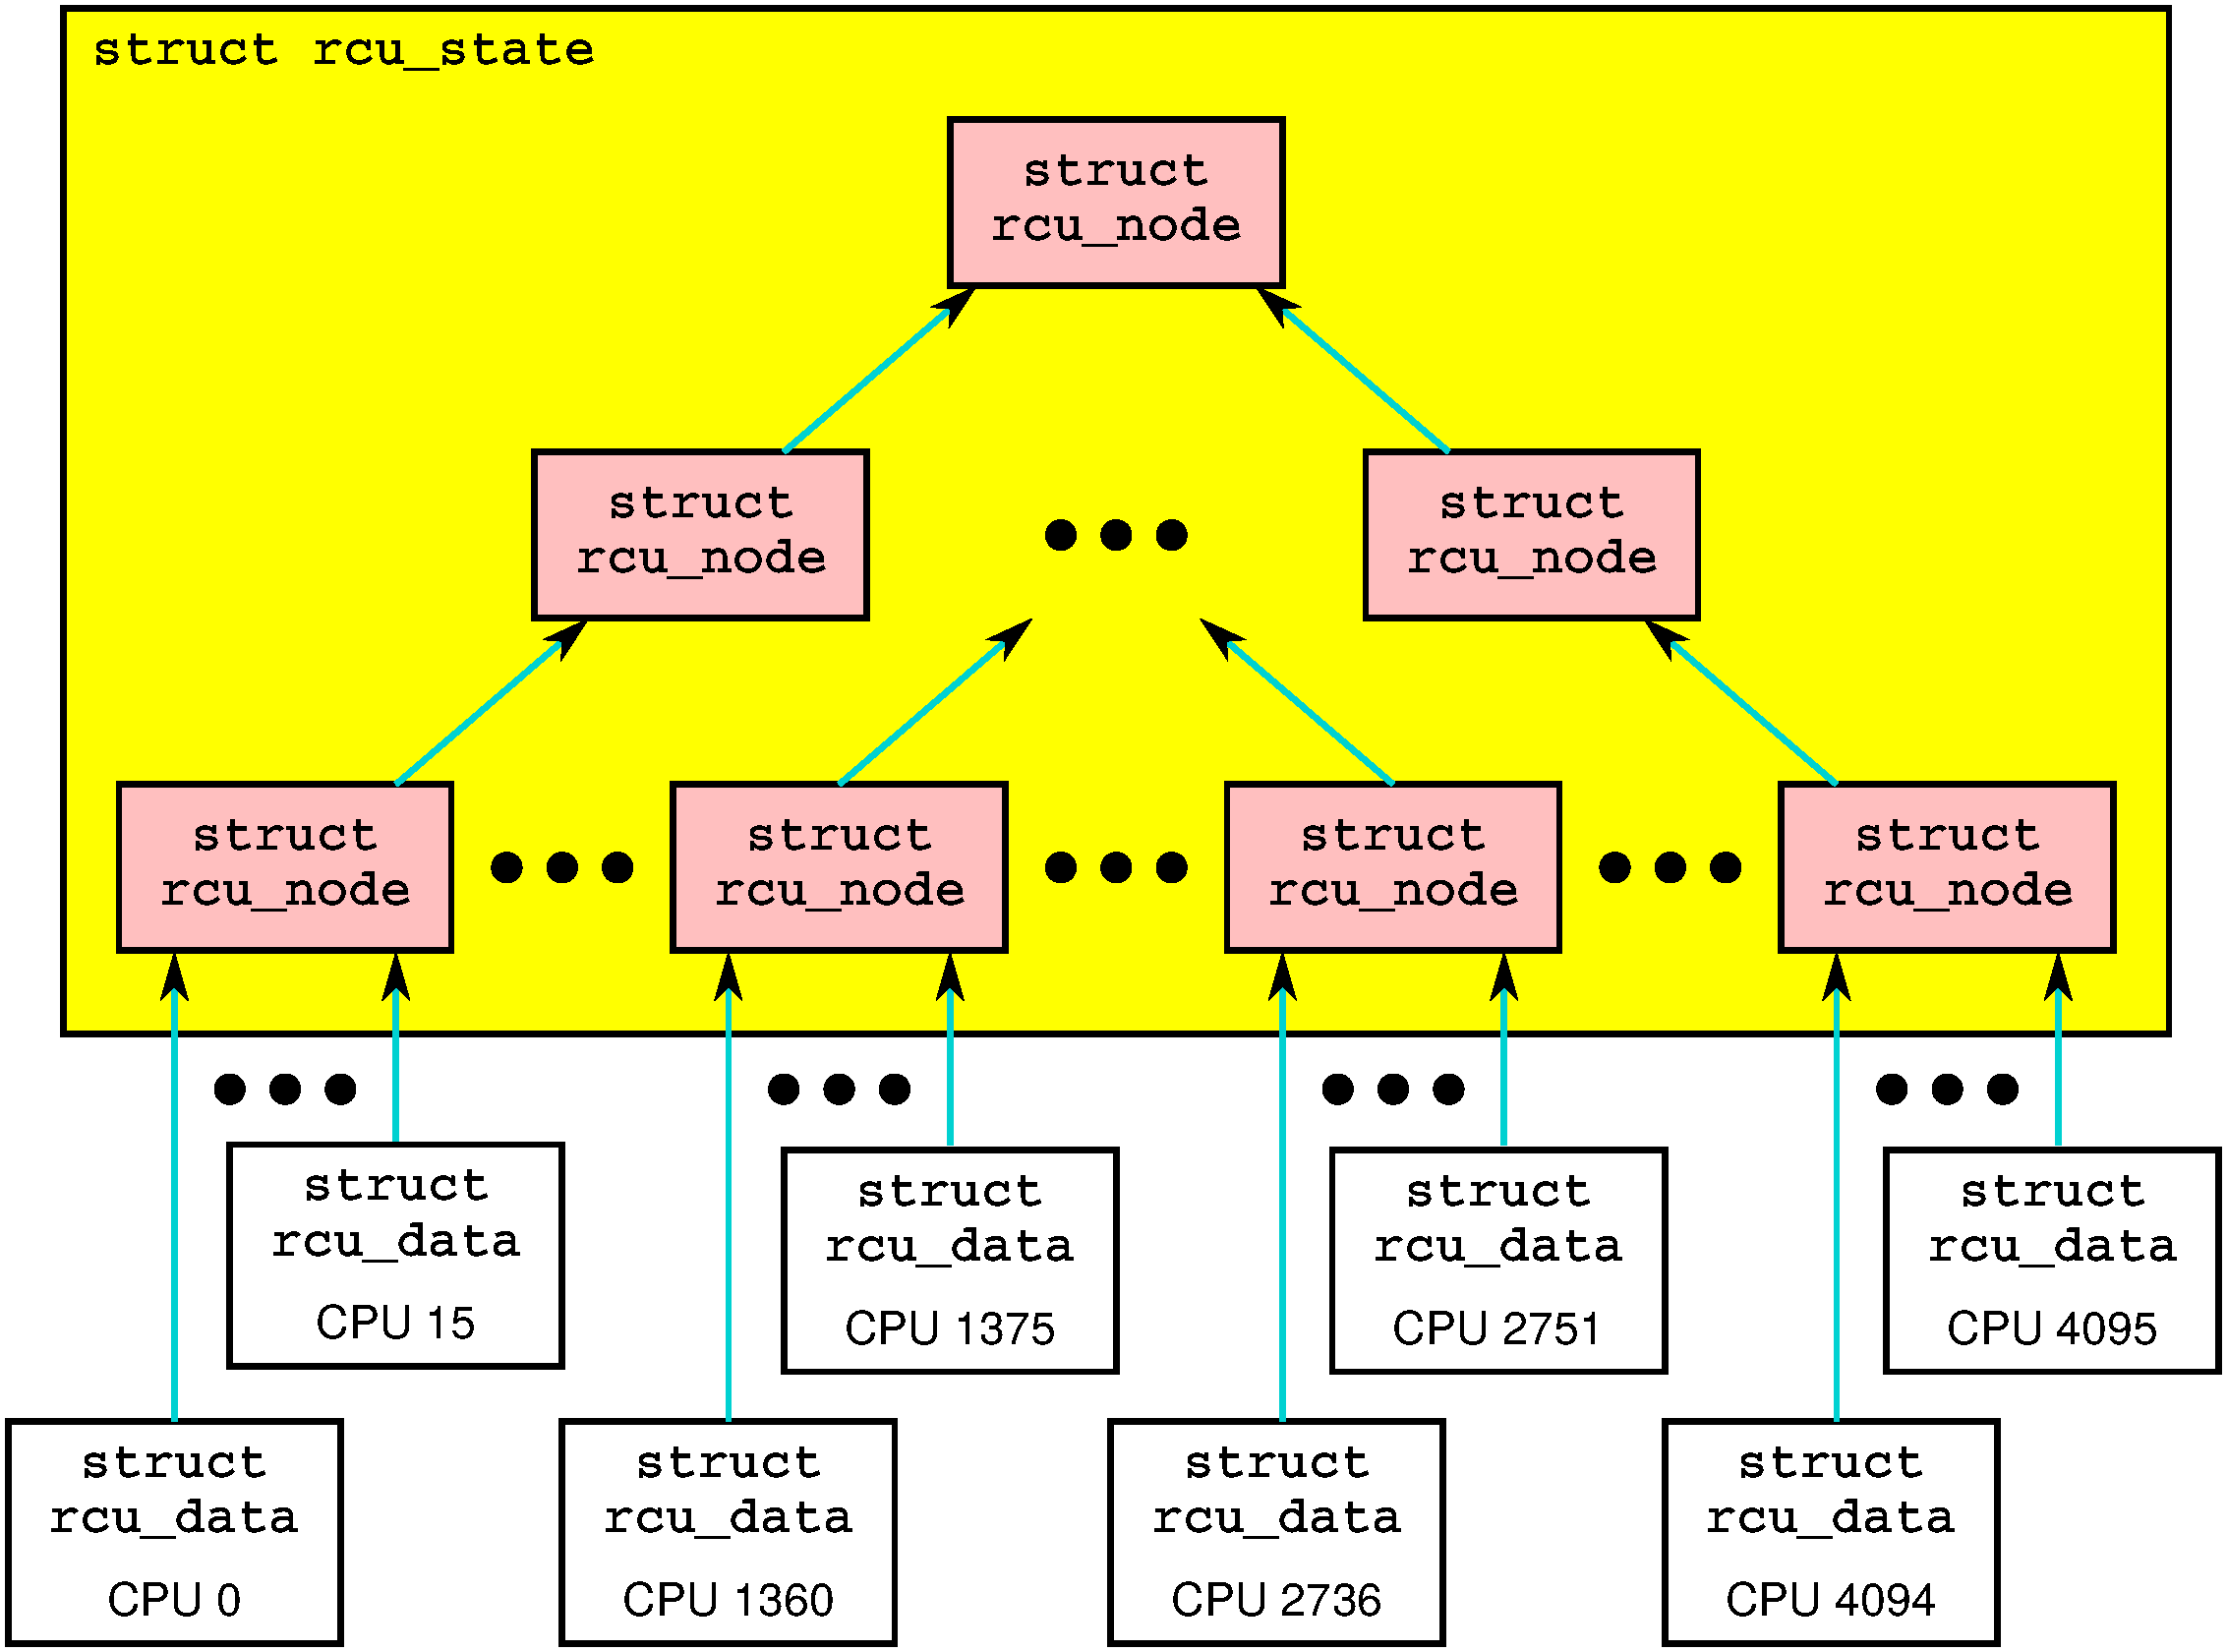
\includegraphics[scale=0.2]{tree_rcu_hierarchy.pdf}
\caption{Иерархия Tree RCU}
\label{fig:tree_rcu_hierarchy}
\end{figure}

Глобальное состояние RCU записывается в структуру \co{rcu_state},
представляющую собой дерево структур \co{rcu_node} с арностью, равной 64
(32 на 32-битных системах). Каждый терминальный узел данного дерева
может иметь ссылки на максимум 64 (32 на 32-битных системах) структуры
RCU's global state is recorded in the \co{rcu_state} structure, which consists of
a tree of \co{rcu_node} structures with a child count of up to 64
(32 in a 32-bit system). Every leaf node can have at most 64 \co{rcu_data},
каждая из которых представляет собой отдельное ядро процессока,
как показано на рисунке~\ref{fig:tree_rcu_hierarchy}.
%
Каждая структура \co{rcu_data} веде учет устойчивых состояний своего ядра,
а \co{rcu_node}-дерево сначала используется для распространения информации
об этих состояниях сначала в направлении корня,
затем --- для распространия информации о grace-периодах в направлении листьев.
%
Информация об устойчивых состояниях передается на родительский уровень
в тот момент времени, когда каждый узел-потомок каждого поддерева данного уровня
уже передал её в корень этого поддерева.
Эта сзема передачи информации позволяет существенно сократить частоту использования
блокировок на верхних уровнях дерева.
%
% Lihao: include this in PhD thesis and the technical report
Например, рассмотрим стандартное \co{rcu_node} дерево для системы с
4{,}096 вычислительными ядрами, имеющее 256 терминальных узлов,
4 внутренних узлов и один корневой узел. В течение данного grace-периода,
каждое ядро сообщит информацию о своем устойчивом состоянии в
соответствующий терминальный узел, но при этом каждому терминальному узлу
будет соответствовать всего 16 соперничающих ядер.
Всего 256 ядер будут пытаться сообщить свои устойчивые состояния внутренним узлам,
при этом всего информация 64 ядер дойдет до каждого из четырех внутренних узов.
Наконец, информация всего четырех ядер может дойти до корневого узла,
что сказывается на его очень низкой частоте блокирования.
Это позволяет использовать данную структуру на очень больших системах.
В частности, актуальная реализация RCU ядра Linux поддерживает
четырехуровневые деревья, что позволяет использовать до
$64^4 = 16{,}777{,}216$ ядрами на 64-битных системах.\footnote{
  В настоящее время четырехуровневые деревья используются при нагрузочном тестировании,
  а трехуровневые находят свое применение на промышленных 4096-ядерных системах.}

\subsubsection{\co{rcu_state} Structure}

\begin{figure}[tbp]
\centering
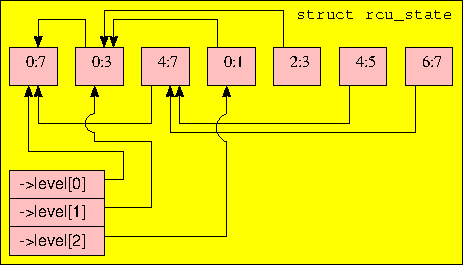
\includegraphics[scale=0.9]{rcu_node_array.pdf}
\caption{Представление дерева структур \co{rcu_node} в виде массива}
\label{fig:rcu_node_array}
\end{figure}

Кажжый реализация RCU имеет свою собственную структуру \co{rcu_state}.
Структура \co{rcu_state} включает в себя массив структур \co{rcu_node},
логически организованных в виде дерева
\co{struct rcu_node node[NUM_RCU_NODES]},
со структурами \co{rcu_data}, присоединенными к его терминальным узлам.
Таким образом, обход этого дерева в ширину сводится линейному проходу по массиву.
Еще один массив структур \co{rcu_node}, \co{*level[NUM_RCU_LVLS]},
используется для указания на самый левый узел каждого уровня дерева,
как показано на рисунке~\ref{fig:rcu_node_array}.

Структура \co{rcu_state} использует поля \co{->gpnum} и \co{->completed}
типа \co{unsigned long} для учета grace-периодов.
Поле \co{->gpnum} используется для отслеживания начала последнего grace-периода,
в то время как \co{->completed} отслеживает окончание последнего grace-периода.
Если значения данных полей одинаковы, то соответствующий RCU находится в состоянии
по умолчанию. Если же значение \co{gpnum} больше, чем \co{completed},
то RCU находится в состоянии grace-периода.
Все прочие комбинации недопустимы.

\subsubsection{\co{rcu_node} Structure}
\label{sec:rcu_node}
Дерево структур \co{rcu_node} регистрирует и распространяет
информацию об устойчивых состояниях от терминальных узлов к корневому,
а также распространяет информацию о grace-периодах в обратном направлении.
%
Структура \co{rcu_node} использует спин-блокировку \co{->lock} для защиты
своих полей. Поле \co{->parent} содержит указатель на струтуру-родителя,
при этом значение данного поля у корневого узла равно \co{NULL}.
Значение поля \co{->level} соответствует, на котором находится данный
узел в дереве, при этом уровень корневого узла равен нулю.
Поле \co{->grpmask} описывает номер бита данного узла в значении поля
\co{->qsmask} узла-родителя.
Поля \co{->grplo} и \co{->grphi} соответствуют наименьшему и наибольшему
порядковому номеру вычислительного ядра, учитываемого данной структурой.

Поле \co{->qsmask} указывает, какие из узлов-потомков еще не сообщили
о своих устойчивых состояниях на данный момент времени.
%
Как и в случае с \co{rcu_state}, структура \co{rcu_node} имеет поля
\co{->completed} и \co{->gpnum}, имеющие такие же значения, как и у родительской
структуры \co{rcu_state}, за исключением начала и конца каждого
grace-периода, когда данные значения копируются из корневого узла.
Значения этих полей могут быть равны друг другу, либо отличаться на единицу.

%\comment{Lihao: comment out the following preemptible RCU contents if we need space.}
%In a preemptible kernel, tasks can be preempted during RCU read-side
%critical sections.
%When an RCU read-side critical section is preempted,
%the preempted task's \co{task_struct} is enqueued onto the \co{->blkd_tasks}
%list in the leaf \co{rcu_node} structure covering the task's CPU.
%That task will remove itself once it reaches the RCU read-side critical
%section's outermost \co{rcu_read_unlock()},
%%
%When the \co{->gp_tasks} pointer is non-\co{NULL}, it references the first
%task blocking the current grace period.
%When a task referenced by \co{gp_tasks} points is removed
%from \co{blkd_tasks}, the pointer will be advanced to the next task on the list,
%or is set to \co{NULL} if there are no more tasks.
%Note that
%tasks blocking the current grace period are queued in the reverse time order.
%Thus, if a task is blocking a grace period,
%all subsequent tasks on the list are blocking the same grace period.
% Lihao: how the tasks are dequeued is described in quiescent state detection
% Lihao: we ignore expedited grace period for now
% Lihao: we don't model priority boosting

\subsubsection{Структура \co{rcu_data}} \label{sec:rcu_data}
Структурв \co{rcu_data} используется для учета устойчивых состояний и
вызова callback'ов связанного вычислительного ядра.
Поскольку доступ к данной структуре осуществляется посредством
связанного вычислительного ядра, нет необходимости выполнять синхронизацию.
Как и в случае со структурой \co{rcu_state}, различные реализации RCU поддерживают
различные виды структур \co{rcu_data}.
% For instance, RCU-sched's
%\co{rcu_sched_state}, RCU-bh's \co{rcu_bh_state} and RCU-preempt's
%\co{rcu_state_p} structures have \co{rcu_data} structures \co{rcu_sched_data},
%\co{rcu_bh_data}, and \co{rcu_data_p}, respectively.
%
Поле \co{->cpu} указывает на связанное вычислительное ядро,
\co{->rsp} --- на связанную структуру \co{rcu_state},
а \co{->mynode} ссылается на соответсвующую терминальную структуру \co{rcu_node}.
Значение поля \co{->grpmask} указывает на позицию структуры \co{rcu_data}
в битовом поле \co{->qsmask} связанной структуры \co{rcu_node}.

Структура \co{rcu_data} содержит поле \co{->qs_pending}, указывающее,
что RCU ожидает получения устойчивого состояния от связанного ядра,
и поле \co{->passed_quiesce}, указывающее на то, что данное ядро уже
прошло через устойчивое состояние.
%
Кроме этого, данная структура также имеет поля \co{->gpnum} и \co{->completed},
значения которых могут отставать от соответсвующих им полей структур
\co{rcu_state} и \co{rcu_node} в нормальном режиме работы ядер процессора.
С другой стороны, если ядра процессора являются заблокированными,
их значения могут оставать на один grace-период от соответсвующих значений
полей структуры \co{rcu_node}.

Поля \co{->gpnum} и \co{->completed} структуры \co{rcu_state} содержат наиболее
актуальные значения и используются для обновления соответствующих полей родительских
структур \co{rcu_node}, что позволяет сравнивать значения данных полей со значениями
этих же полей структур \co{rcu_node} для фиксации факта начала нового grace-периода.
Эта схема позволяет вычислительным ядрам обнаруживать границы grace-периодов
без использования блокировок.
%
Структруа \co{rcu_data} управляет RCU callback'ами с помощью
структуры данных, известной как четырехсегментный
список~\cite{LaiJiangshan2008NewClassicAlgorithm}.

% Lihao: but we need to carefully manage the numbers of each node as the consequences of
% using a quiescent state in a wrong grace period can be quite serious.
% Paul: Indeed!  And the grace-period initialization (rcu_gp_init()) and
% cleanup (rcu_gp_cleanup()) code first updates the rcu_state structure and
% then the rcu_node structures in breadth-first order to avoid such
% consequences.  In addition, cleanup propagates ->completed completely
% and only then is ->gpnum propagated for the new grace period.  Attempting
% to "optimize" this to propagate ->completed and ->gpnum changes in one
% pass results in nasty race conditions caused by different CPUs believing
% that different active grace periods are in effect.  Very low probability,
% but -very- nasty.

% Lihao: we don't model dyntick-idle handling
% Lihao: include this in the technical report
\begin{figure}[tbp]
\centering
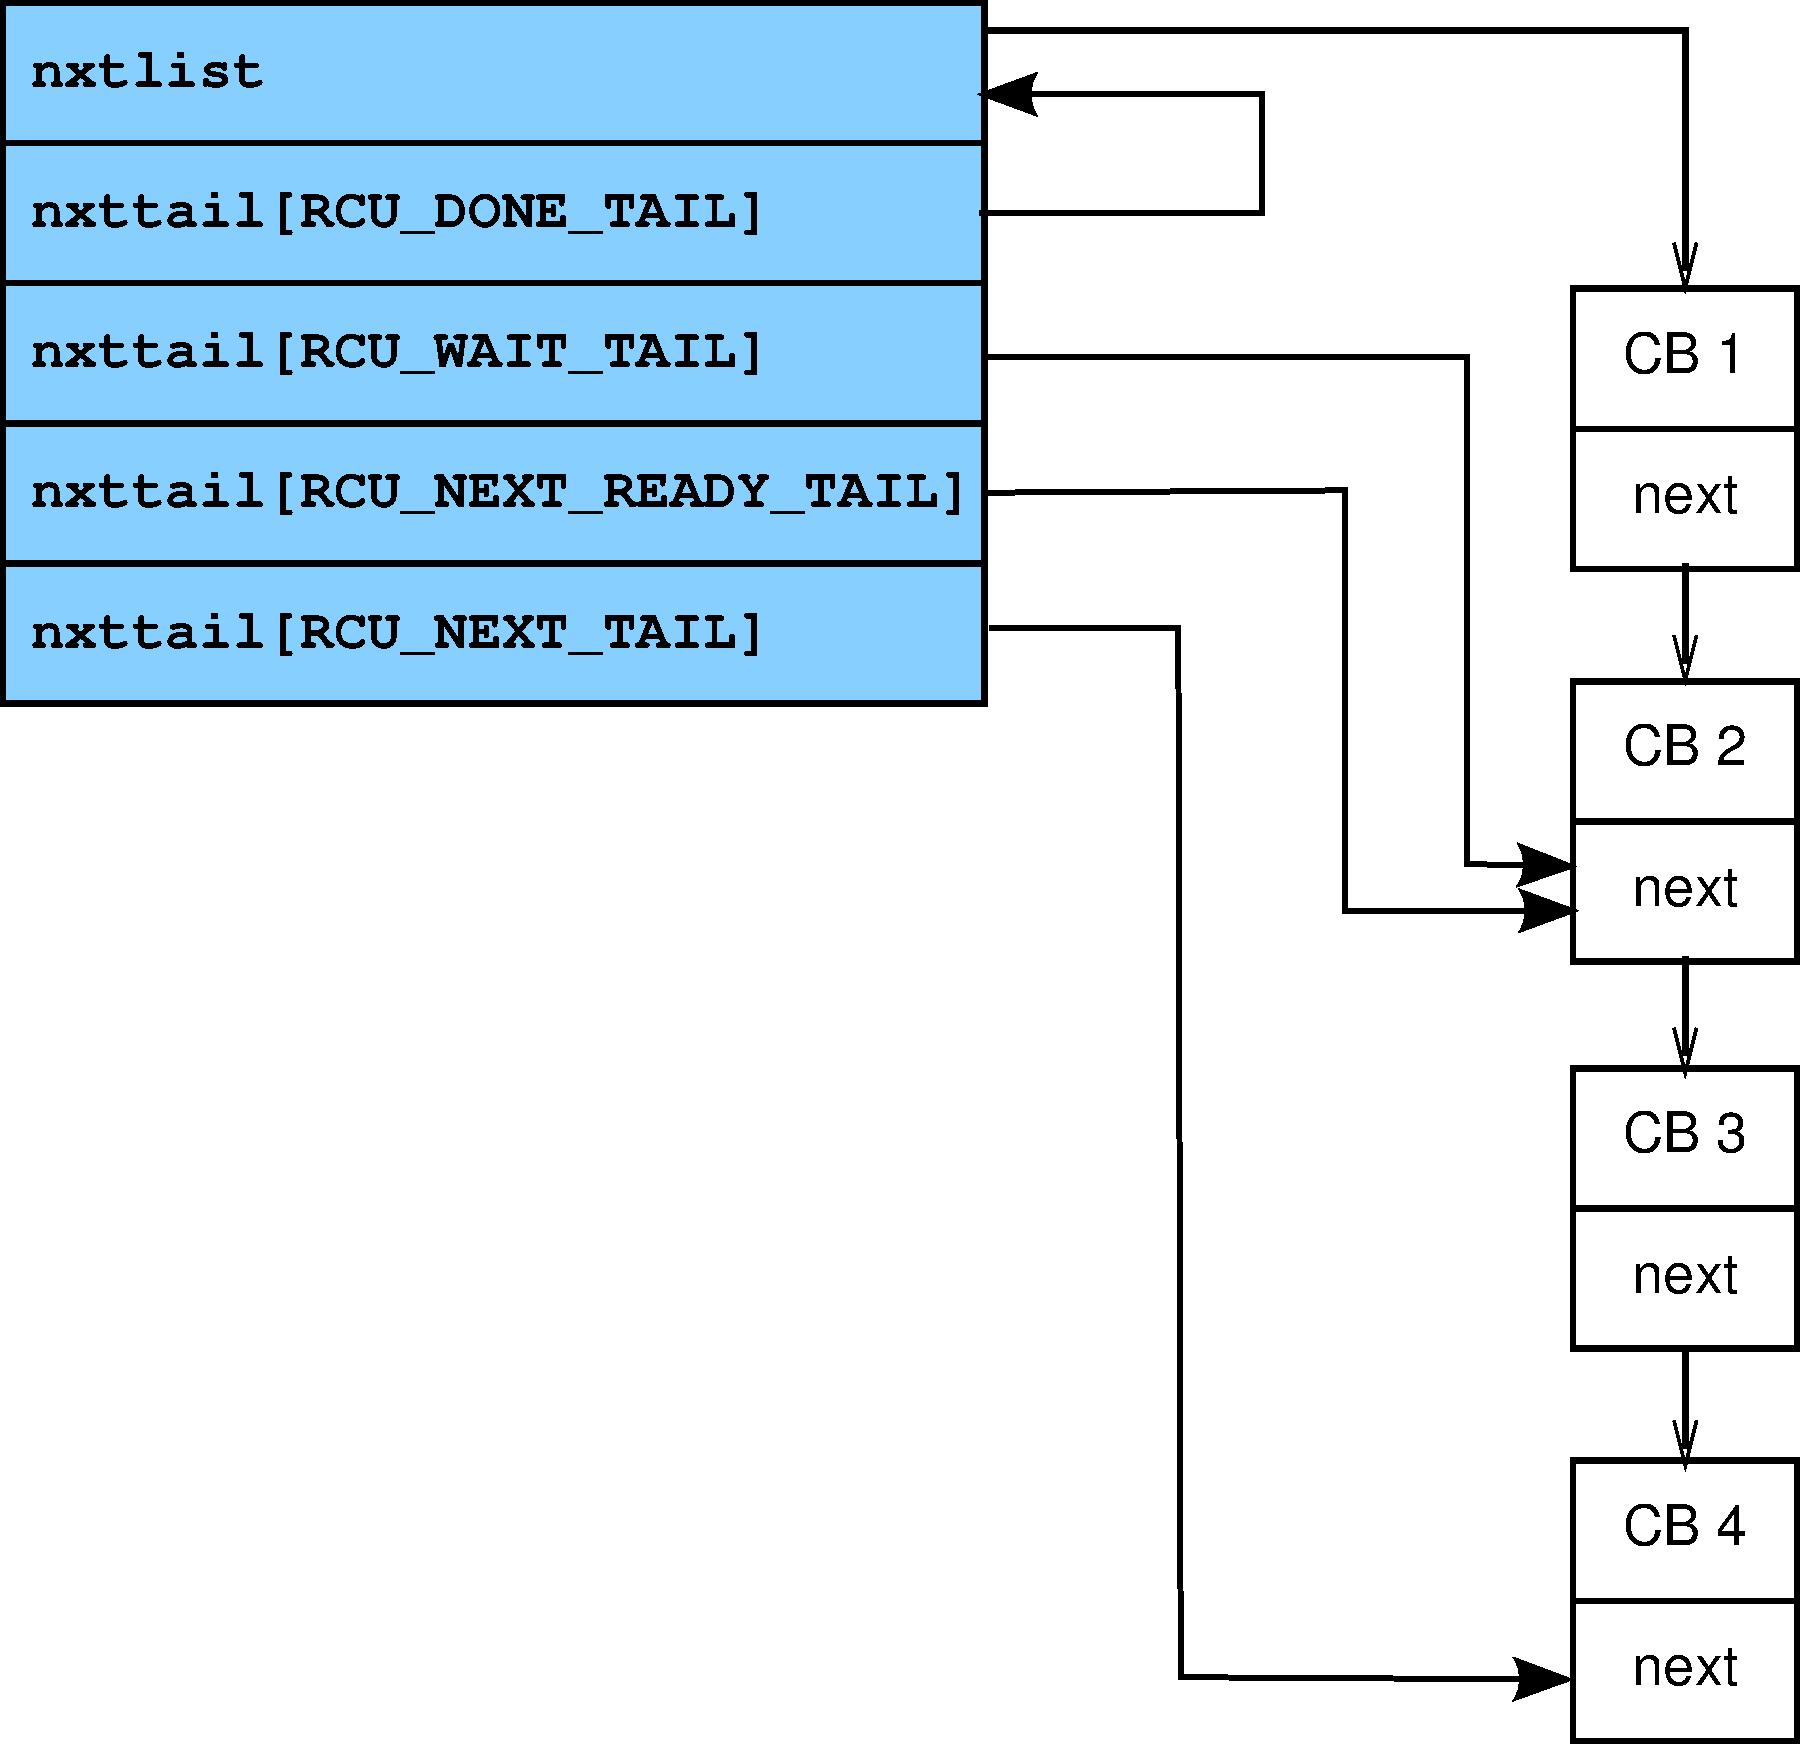
\includegraphics[scale=0.25]{rcu_data_callbacks.pdf}
\caption{Callback Queuing in \co{rcu_data}}
\label{fig:rcu_data_callbacks}
\end{figure}

%\comment{Lihao: since we don't model callbacks, only describe them briefly and add a reference
%to save space for the experiments section which is the main contribution of this paper. 
%Do the same for discussion of preemptible RCU.}
\subsubsection{RCU Callbacks}
The \co{rcu_data} structure manages RCU callbacks using a \co{->nxtlist}
pointer tracking the head of the list and an array of \co{->nxttail[]}
tail pointers that form a four-segment list of
callbacks~\cite{LaiJiangshan2008NewClassicAlgorithm}, with
each element of the \co{->nxttail[]} array referencing the tail of the
corresponding segment, as shown in Figure~\ref{fig:rcu_data_callbacks}.
The segment ending with \co{->nxttail[RCU_DONE_TAIL]} (the ``\co{RCU_DONE_TAIL}
segment'') contains callbacks
handled by a prior grace period that are therefore ready to be invoked.
The \co{RCU_WAIT_TAIL} and \co{RCU_NEXT_READY_TAIL} segments 
contain callbacks waiting for the
current and the next grace period, respectively.
Finally, the \co{RCU_NEXT_TAIL} segment contains
callbacks that are not yet associated with any grace period.
%
The \co{->qlen} field counts the total number of callbacks, and
the \co{->blimit} field specifies the maximum number of RCU callbacks
that may be invoked at a given time, thus limiting response-time
degradation due to long lists of callbacks.\footnote{
	Workloads requiring aggressive real-time guarantees should use
	callback offloading, which is outside of the scope of this paper.}

Back in Figure~\ref{fig:rcu_data_callbacks}, the
\co{->nxttail[RCU_DONE_TAIL]} array element references \co{->nxtlist}, 
which means none of the callbacks are ready to invoke.
The \co{->nxttail[RCU_WAIT_TAIL]} element references callback 2's \co{->next}
pointer, meaning that callbacks CB~1 and CB~2 are waiting for the current
grace period.
The \co{->nxttail[RCU_NEXT_READY_TAIL]} element references that same \co{->next}
pointer, meaning that no callbacks are waiting for the next grace period. 
Finally, the callbacks between the \co{->nxttail[RCU_NEXT_READY_TAIL]} and
\co{->nxttail[RCU_NEXT_TAIL]} elements (CB~3 and CB~4)
are not yet assigned to a specific grace period.
The \co{->nxttail[RCU_NEXT_TAIL]} element always references either
the last callback or, when the entire list is empty, \co{->nxtlist}.

Cache locality is promoted by invoking callbacks on the CPU that registered
them.
For example, RCU's update-side primitive 
\co{synchronize_rcu()} appends callback \co{wakeme_after_rcu()} to the end
of the \co{->nxttail[RCU_NEXT_TAIL]} list in the current CPU 
(Section \ref{sec:update_api_impl}). 
They are advanced one segment towards the head of the list (via \co{rcu_advance_cbs()}) 
when the CPU detects the current grace period has ended, which is indicated 
by the \co{->completed} field of the CPU's \co{rcu_data} structure being one
smaller than its counterpart in the corresponding leaf \co{rcu_node} structure.
The CPU also periodically merges the \co{RCU_NEXT_TAIL} segment into the
\co{RCU_NEXT_READY_TAIL} segment by calling \co{rcu_accelerate_cbs()}.
In a few special cases, the CPU merges the \co{RCU_NEXT_TAIL} segment
into the \co{RCU_WAIT_TAIL} segment, bypassing the \co{RCU_NEXT_TAIL}
segment.
This optimization applies when the CPU is starting a new grace period.
It does \emph{not} apply when a CPU notices a new grace period
because that grace period might well have started before
the callbacks were added to the \co{RCU_NEXT_TAIL} segment.
%\comment{Lihao: why can't we invoke *all* callbacks when starting a new 
%grace period? Isn't it true that all pre-existing read-side critical
%sections, i.e.~those start before callbacks are registered in \co{->nxttail} 
%(in particular \co{wakeme_after_rcu} in \co{->nxttail[RCU_NEXT_TAIL]}), 
%have finished?}
%\comment{Paul: In theory, we could, but in practice doing this would
%have several disadvantages:
%(1) All callbacks would be invoked by the grace-period kthread, and
%large systems could generate more callbacks than a single CPU could
%keep up with, which would delay subsequent grace periods and possibly
%even run the system out of memory.
%(2) Running all the callbacks at once could degrade real-time response.
%(3) Running callbacks on a different CPU than the one that registered
%them would decrease locality, increasing cache-miss rates, thus degrading
%performance.
%(4) This would require that atomic instructions be used when registering
%callbacks (as they are for no-CBs CPUs), further degrading performance.
%In addition, we could only invoke callbacks in the \co{RCU_NEXT_TAIL}
%segment, because callbacks in the later segments
%(\co{RCU_NEXT_READY_TAIL}, \co{RCU_WAIT_TAIL}, and
%\co{RCU_DONE_TAIL} might well have been queued \emph{after} the
%recently-completed grace period started.}
%
This is a deliberate design choice: It is more important for the CPUs
to operate independently (thus avoiding contention and synchronization
overhead) than it is to decrease grace-period latencies.
In those rare occasions where low grace-period latency is important,
the \co{synchronize_rcu_expedited()} should be used.
This function has the same semantics as does \co{synchronize_rcu()},
but trades off efficiency optimizations in favor of reduced latency.
% Lihao: this is where the callback of RCU's update API register? 
% Paul: Yes, call_rcu() appends the callback to the end of the current
% CPU's RCU_NEXT_TAIL list.  Ignoring callback offloading for the moment.
% Lihao: we don't model QS forcing and offline CPUs
% Paul: Nor are you modeling callback offloading.  Which is fine, just calling
% it out.  ;-)

Each RCU callbacks is an \co{rcu_head} structure which has a
\co{->next} field that points to the next callback on the list and
a \co{->func} field that references the function to be invoked at the
end of an upcoming grace period.



